\chapter{Discrete Routing, Continuous Offspring Geography, and Background Nuisance in New Zealand}

In the tables, $I_{\mathrm{d,g}}$ denotes distance excitation with global stress (the saved identifier \texttt{I\_distance\_globalG}). A stacked mantissa and power of ten form one scientific-notation value; their full displayed precision is retained.
\label{ch:nz-spatial}
\section{From regional aggregation to matched spatial forecasts}
The successive studies below turn the locality question into matched predictive comparisons. They progress from three labelled zones (C1), through a conserved cross-zone mixing law (W), finite-cell distance allocation (D), and continuous-area offspring density (S), to a joint temporal--spatial/background factorial. These stages reuse the historical windows; their gains cannot be concatenated into an independent replication count. The regional algebra motivates the completed comparisons without identifying a geological mechanism.

\paragraph{Execution provenance.}
This chapter retains the original spatial and background-extension fits and numerical audits. The later selected-state replay recomputes the declared likelihoods using the recovered cached features and reconciles the common-space and partition comparisons. It does not rerun optimizer searches. The fresh frozen diagnostic and autonomous fits in Chapter~\ref{ch:observed} are separate computations.

The completed spatial programme compared, on the same region-labelled observations, three deliberately matched candidates: no inhibition, pooled inhibition across regions, and local inhibition. For a given regional history, the motivating schematic intensities are
\begin{align}
  \lambda_k^{(0)}&=B_k+H_k, \label{eq:locality-none}\\
  \lambda_k^{(\mathrm{pool})}
    &=B_k\exp\!\left(-\eta\sum_jG_j\right)+H_k, \label{eq:locality-pooled}\\
  \lambda_k^{(\mathrm{local})}
    &=B_k\exp(-\eta G_k)+H_k, \label{eq:locality-local}
\end{align}
where \(H_k\) includes the trigger amplitude and must be defined identically across alternatives. A fair comparison matches spatial backgrounds, triggering families with a serious Omori baseline, mark and history rules, observation rules, and fitting effort. With region label \(r_i\) for event \(i\), every candidate uses the same joint score
\begin{equation}
 \ell=\sum_i\log\lambda_{r_i}(t_i-)
      -\sum_k\int_0^T\lambda_k(t)\,\dif t
      +\sum_i\log f(m_i).
 \label{eq:proposed-spatial-score}
\end{equation}
The integrals include quiet regions and quiet intervals. Omitting them would reward or penalize models according to event allocation without accounting for exposure. Alternatively, candidates must be marginalized to the same label-discarded observations; a label-aware likelihood and a label-discarded likelihood cannot be ranked as if they used the same data event.


The subsequent stages declare their own background and geometry recipes. A later replay may differ at solver precision from an older sealed result; it does not replace that result. Throughout this chapter, an ``Event'' column is the point-event logsum contribution and ``Compensator'' is the signed contribution $C=-E$. For discrete zones/cells, the point intensity is with respect to counting measure; continuous comparisons below first put every arm on the same projected-area measure.

\section{C1: region-labelled local and global controls}

C1 supports localizing excitation for time-zone prediction, but does not support adding local stress inhibition to that localized excitation model. All three folds, four models, 12 case fits and 96 prescribed starts completed. The independent raw-row audit passed, reconciling 114 candidates and 96 solver returns; saved near-optimal forecasts passed the declared stability gate. The catalogue and historical authorities were preserved.

\subsection{Separate timing from zone prediction}

On the 612 held-out targets, local excitation beats global excitation by 349.786446 joint nats (+0.571546481 nats/event), positive in all three folds. Of this gain, 347.958257 nats comes from conditional-zone prediction and only 1.828190 nats from regional timing. Joint gains are +105.104546, +119.000978 and +125.680922 nats; timing differences are -2.083237, +1.797562 and +2.113864. The strong joint result therefore concerns predicting which of three fixed latitude bands receives the next event. It is not evidence of a comparably large improvement in event timing or of continuous-location forecast skill.

At the same parameters, local E0 and global E0 have exactly the same regional ground intensity and compensator. Their conditional-zone factors differ, so selecting each by full time-zone training NLL produces different fitted parameters and modestly different timing forecasts. The observed timing difference does not contradict the fixed-parameter identity.

Local inhibition also beats global inhibition strongly: +364.573096 joint nats (+0.595707674 nats/event), including +17.936860 regional-timing and +346.636237 conditional-zone nats. Both joint and timing differences are positive in all three folds. This comparison includes both localized triggering and localized stress, and the poor globally inhibited baseline. It does not establish the value of inhibition beyond a matched local excitation model.

\subsection{The matched inhibition result remains negative}

Adding local inhibition to local excitation loses 3.399761 joint nats (-0.005555164 nats/event): -2.077741 regional timing and -1.322020 conditional zone. Fold differences are -0.207862, -3.191896 and approximately zero (-0.000003) nats. The last difference is below the 0.0001-nat score-reconciliation tolerance and the selected eta is exactly zero; it should be described as a numerical tie rather than a substantive third forecast loss.

The local inhibitory fit lowers training NLL by approximately 0.112071, 1.061892 and zero nats in Folds 0-2, respectively, yet none yields a substantive held-out gain. These are modest training improvements of a nested bounded fitting procedure, not evidence for a nonzero physical depletion parameter.

Global inhibition loses 18.186411 nats (-0.029716357 nats/event). The difference of matched inhibition contrasts is therefore +14.786650 nats (+0.024161193 nats/event): localization makes the inhibitory penalty much less severe, while the local incremental inhibition contrast remains negative. This descriptive difference is positive in Folds 0 and 2, negative in Fold 1. It is not a causal difference-in-differences design.

\subsection{Fold 0 and proper exposure accounting}

Fold 0's global inhibitory contrast is -16.988735 nats, decomposed into -33.904743 event and +16.916008 compensator nats. The matched local inhibitory contrast is -0.207862 nats: -3.000762 event and +2.792900 compensator nats. Regional timing improves from a -16.988735 global inhibitory penalty to a -0.831697 local inhibitory penalty; the local conditional-zone contribution is +0.623835 nats.

The proper Fold 0 local inhibitory score differences by zone are +0.289381 south, -0.141682 central and -0.355561 north. Their sum gives -0.207862. Across all three folds, the matched local inhibitory differences are negative in each zone: -1.199738, -1.134201 and -1.065822 nats. These are full zone contrasts with their own valid integrated exposures, not event-only geographical summaries.

The large local-versus-global joint gains cannot be reduced to a positive event term everywhere. For example, Fold 0 local E0 has a negative central-zone event contrast (-2.324219 nats), offset by a +17.184730 compensator contribution, giving a +14.860511 central-zone total. Quiet exposure and all-zone compensators are essential to the result.

\subsection{Parameters and historical reconciliation}

The selected global eta values are 1.451113, 0.230849 and 0.116715; local eta values are 0.374699, 0.517222 and 0. Local eta is smaller in Folds 0 and 2 but larger in Fold 1. There is no uniform shrinkage result. Local and global stress histories also differ in scale and composition, so eta alone is not a directly comparable measure of physical stress strength. No selected coordinate hits a restrictive box boundary except the local eta=0 boundary in Fold 2.

The fresh global inhibitory contrasts reproduce Stage A's global raw contrasts to numerical precision: Fold 0 shifts by about 1e-11 nats, Fold 1 by +0.000013869 and Fold 2 by -0.000009878. Fixed-parameter global reduction was independently verified; these tiny separately optimized fit shifts are not failures of that identity. Historical Iteration28's -16.517557 Fold 0 contrast belongs to its own fitted/nuisance recipe and remains a separate authority.

The old five-degree cell crosswalk regroups event log-intensity ratios only. C1 defines three zone intensities, without a within-zone cell probability model; consequently cell compensators and cell full likelihoods are undefined. Proper zone compensators remain separate. Historical cell event penalties are retained with their source hashes and are not spliced into new denominators.

\subsection{Delimited conclusion}

The useful result is strong retrospective categorical-zone prediction from localized triggering, with a small mixed-sign timing benefit for local E0. Localizing the whole inhibitory procedure largely removes the catastrophic global inhibition penalty, but the matched local inhibitory extension still adds no held-out value. This supports retaining \modeltag{E0}{local} as the better of these declared local procedures; it does not demonstrate physical stress inhibition or identify a causal spatial mechanism.

The result applies to three predeclared latitude bands, omega=0, fixed r=0.7 and the retained ML law on one previously examined regional catalogue. Training-only pi and beta were frozen for test; observed history updated predictably. No event-iid confidence interval, Wilks boundary test, global-optimum certificate, new partition, kernel search, C2 or other model stage follows from this review.

Evidence: results/\allowbreak{}\allowbreak{}analysis/summary.json; methods/\allowbreak{}\allowbreak{}observed\_\allowbreak{}saved\_\allowbreak{}audit.json; results/\allowbreak{}\allowbreak{}analysis/historical\_\allowbreak{}reconciliation.json; results/\allowbreak{}\allowbreak{}analysis/cell\_\allowbreak{}event\_\allowbreak{}crosswalk.json; design/spatial\_\allowbreak{}zone\_\allowbreak{}counts.json; protocol\_\allowbreak{}observed\_\allowbreak{}v1.json. This interpretation introduces no numerical refit or pinned-source change.

\subsection{C1: complete audited comparisons}

All three folds, four models (12 case fits), and 96 prescribed starts are complete. The same 612 held-out targets are scored once per model. The interpretation in Section~\ref{sec:empirical-interpretation} applies.

\begingroup\scriptsize\setlength{\tabcolsep}{2pt}\renewcommand{\arraystretch}{1.18}
\begin{longtable}{@{}>{\raggedright\arraybackslash}p{0.1251\textwidth}>{\raggedright\arraybackslash}p{0.1251\textwidth}>{\raggedright\arraybackslash}p{0.1251\textwidth}>{\raggedright\arraybackslash}p{0.1251\textwidth}>{\raggedright\arraybackslash}p{0.1251\textwidth}>{\raggedright\arraybackslash}p{0.1251\textwidth}>{\raggedright\arraybackslash}p{0.1251\textwidth}@{}}
\toprule
{}Comparison & Regional timing & Conditional zone & Magnitude & Joint nats & Nats/event & Positive folds \\
\midrule\endfirsthead
\toprule
Comparison & Regional timing & Conditional zone & Magnitude & Joint nats & Nats/event & Positive folds \\
\midrule\endhead
\midrule\multicolumn{7}{r}{\emph{Continued on next page}}\\
\endfoot
\bottomrule\endlastfoot
{}\modeltag{E0}{local}\allowbreak{}-\allowbreak{}\modeltag{E0}{global} & 1.82819 & 347.958 & 0 & 349.786 & 0.571546 & 3/3 \\
{}\modeltag{I0}{local}\allowbreak{}-\allowbreak{}\modeltag{I0}{global} & 17.9369 & 346.636 & 0 & 364.573 & 0.595708 & 3/3 \\
{}\modeltag{I0}{local}\allowbreak{}-\allowbreak{}\modeltag{E0}{local} & -2.07774 & -1.32202 & 0 & -3.39976 & -0.00555516 & 0/3 \\
{}\modeltag{I0}{global}\allowbreak{}-\allowbreak{}\modeltag{E0}{global} & -18.1864 & \shortstack[r]{$-5.11591$\\$\times10^{-13}$} & 0 & -18.1864 & -0.0297164 & 0/3 \\
{}(\modeltag{I0}{local}\allowbreak{}-\allowbreak{}\modeltag{E0}{local})-(\modeltag{I0}{global}\allowbreak{}-\allowbreak{}\modeltag{E0}{global}) & 16.1087 & -1.32202 & 0 & 14.7866 & 0.0241612 & 2/3 \\
\end{longtable}\endgroup

% Audit-table relocation: app:audit10-c1
The complete C1 per-fold contrasts and exact zone decompositions are retained in Appendix~\ref{app:audit10-c1}.

\subsection{Scope}

K=3 fixed latitude zones, raw local stress, fixed ML excitation and r=.7, omega=0. Background proportions and magnitude nuisance use training only. Local triggering and local inhibition are compared with matched global/local excitation controls. Joint gains can come from zone prediction without improved regional timing; the two components must not be conflated.

The C1 model does not define within-zone cell probabilities, so cell event crosswalks have no invented cell compensators. Full compensator differences are reported per zone. Historical Iteration28 cell event penalties and recipe differences are retained separately in historical\_\allowbreak{}reconciliation.json.

All comparisons are retrospective on previously examined chronological windows. The common inferential and optimization boundaries in Section~\ref{sec:empirical-interpretation} apply. No follow-up model/kernel/productivity search or other stage was run.

\section{W: conserved cross-zone redistribution}

W supports a small training-estimated global redistribution component in the otherwise local excitation model for zone prediction. It does not support an incremental inhibitory extension or a direct timing benefit from the mixing weight. All 27 case fits and 216 prescribed starts completed; the independent raw-row audit passed, checking 279 candidates and 216 solver returns. Reported differences use 612 targets and common magnitude scores cancel.

\subsection{Excitation mixing improves the joint score through zone prediction}

Free-omega excitation improves on purely local excitation by 10.553372 joint nats (+0.017244071 nats/event), positive in all three held-out windows: +2.293398, +8.176718 and +0.083256 nats. Its conditional-zone gain is +13.789492 nats, while regional timing worsens by 3.236121 nats. Timing differences are +0.865688, -0.561462 and -3.540347 nats. The joint improvement should therefore be described as a categorical-zone forecast improvement with a net timing cost.

Selected excitation \(\omega\) values are 0.046125, 0.045172 and 0.044339. These are weights on a globally redistributed trigger component; they are not literal cross-zone offspring probabilities. The globally redistributed component can also return to the parent's own zone, so a parent's actual cross-zone allocation is \(\omega(1-\pi_{z_j})\), where \(z_j\) is the parent's zone. No physical transfer rate is identified by these fitted routing weights.

The free model's training NLL gains against omega0 are approximately 2.163997, 4.867366 and 13.271381 nats. Exact completed endpoint floors preserve the nested training comparison, and all prescribed starts and near-optimal forecast checks passed. Three similar estimates from overlapping training prefixes do not provide an independent replication or confidence interval for a physical mixing parameter.

Free excitation beats global excitation by 360.339778 joint nats (+0.588790487 nats/event), with +361.747747 conditional-zone nats and -1.407969 timing nats. This chiefly retains the large spatial prediction benefit already seen in C1, with an additional modest gain over the strictly local endpoint.

\subsection{Omega has no direct timing effect}

For either fixed stress choice and the same remaining parameters,

\begin{equation}\sum_z\lambda_z=\sum_z\pi_z e^{a+d x_{\mathrm{trend}}(t)-\eta G_z^{\rm stress}}+nH_{\rm global}.\end{equation}

Omega cancels because excitation allocation is column-stochastic. This holds for E and both local/global-stress I families. Ground likelihood and total compensator are omega-invariant at fixed (a,d,n,eta). The observed timing changes arise indirectly because full time-zone training refits those other coordinates. They do not overturn the shared-kernel timing-invariance result or establish direct improvement in event timing from cross-zone redistribution.

\subsection{Matched free inhibition remains negative}

With omega free in both matched models, local-stress inhibition loses 3.637297 joint nats (-0.005943296 nats/event) against excitation: -2.292422 timing and -1.344875 conditional-zone nats. Fold differences are +0.087297, -3.232617 and -0.491977 nats. Even the small Fold 0 joint gain combines worse timing (-0.704286) with better zone prediction (+0.791583). Regional timing is worse in all three windows.

Global-stress inhibition loses 12.887727 joint nats (-0.021058377 nats/event): -11.593479 timing and -1.294248 zone nats. Fold differences are -11.191948, +0.639379 and -2.335157 nats. Most of its aggregate loss remains in Fold 0. Local-stress inhibition outperforms global-stress inhibition in the free-omega comparison by 9.250429 nats, positive in two windows, but neither improves on matched excitation overall.

The selected free local-stress eta values are 0.281470, 0.579390 and 0.059749, with omega near 0.044-0.045. Free global-stress eta values are 0.910443, 0.133890 and 0.162321; their omega values are 0.068905, 0.048547 and 0.046997. These are fitted constrained prediction coordinates under different stress histories, not directly comparable physical stress strengths or a causal explanation of the losses.

\subsection{The factorial endpoints prevent a blanket localization claim}

At fixed local excitation (omega0), global-stress inhibition loses only 1.005026 aggregate nats, whereas local-stress inhibition loses 3.399764 nats. Thus local stress is not uniformly the better stress choice. The global-stress eta is 0.068165 in Fold 0 and exactly zero in Folds 1 and 2; its tiny positive score differences in those latter windows are numerical ties, not meaningful forecast wins.

At fixed global excitation (omega1), local-stress eta is exactly zero in all three windows. Its aggregate score difference from excitation is -0.000031725 nats, below the 0.0001-nat saved-score reconciliation tolerance, and should be treated as a nested numerical tie. Global-stress inhibition at that same excitation endpoint loses 18.186431 nats, including -16.988727 in Fold 0.

The factorial result is an interaction among excitation routing, stress choice and joint nuisance refitting. It does not justify a universal statement that localizing stress rescues inhibition. Much of the earlier local-versus-global improvement is attributable to excitation routing and conditional-zone forecasting. The raw positive-window counters in the audit retain arithmetic signs; eta0 differences of order1e-5 or1e-6 are not scientific evidence for an inhibitory gain.

\subsection{Proper exposure and conclusion}

All score contrasts include complete zone compensators. For example, Fold 0 free-local-inhibition versus free excitation has an event contribution of -2.002970 nats and a compensator contribution of +2.090266, giving +0.087297. Event penalties alone would give the wrong sign. No cell-within-zone score is present in this three-zone W stage; its full score is timing plus conditional zone plus common magnitude.

The delimited result favors free-omega excitation for categorical-zone forecasting among the declared W procedures, while the incremental local/global inhibitory alternatives remain negative overall. There is no direct omega timing effect, physical stress-transfer claim, event-iid confidence interval, Wilks boundary inference or global-optimum certificate.

D's model support, smoothing, distance grid, synthetic laws and selection rules were frozen before W outcomes. This interpretation changes none of them. Its historical admission depended on engineering correctness and protected resource/audit reserves; a positive W result was not an admission condition. The same held-out events were reused in D, rather than forming a fresh independent validation catalogue.

Evidence: results/\allowbreak{}\allowbreak{}W/analysis/\allowbreak{}\allowbreak{}summary.json; methods/\allowbreak{}\allowbreak{}W\_\allowbreak{}observed\_\allowbreak{}saved\_\allowbreak{}audit.json; protocol\_\allowbreak{}W\_\allowbreak{}observed.json; reports/\allowbreak{}\allowbreak{}W\_\allowbreak{}decision\_\allowbreak{}report.md. No new fit, source modification or extension was performed for this interpretation.

\subsection{W: complete audited comparisons}

All declared procedures and starts resolved. Source and audit bind this report to the frozen protocol. The interpretation in Section~\ref{sec:empirical-interpretation} applies.

\begingroup\scriptsize\setlength{\tabcolsep}{2pt}\renewcommand{\arraystretch}{1.18}
\begin{longtable}{@{}>{\raggedright\arraybackslash}p{0.1251\textwidth}>{\raggedright\arraybackslash}p{0.1251\textwidth}>{\raggedright\arraybackslash}p{0.1251\textwidth}>{\raggedright\arraybackslash}p{0.1251\textwidth}>{\raggedright\arraybackslash}p{0.1251\textwidth}>{\raggedright\arraybackslash}p{0.1251\textwidth}>{\raggedright\arraybackslash}p{0.1251\textwidth}@{}}
\toprule
{}Comparison & Regional timing & Conditional zone & Within-zone cell & Joint nats & Nats/event & Positive folds \\
\midrule\endfirsthead
\toprule
Comparison & Regional timing & Conditional zone & Within-zone cell & Joint nats & Nats/event & Positive folds \\
\midrule\endhead
\midrule\multicolumn{7}{r}{\emph{Continued on next page}}\\
\endfoot
\bottomrule\endlastfoot
{}\modeltag{E}{wfree}\allowbreak{}-\allowbreak{}\modeltag{E}{w0} & -3.23612 & 13.7895 & 0 & 10.5534 & 0.0172441 & 3/3 \\
{}\modeltag{E}{wfree}\allowbreak{}-\allowbreak{}\modeltag{E}{w1} & -1.40797 & 361.748 & 0 & 360.34 & 0.58879 & 3/3 \\
{}\modeltag{Ilocal}{wfree}\allowbreak{}-\allowbreak{}\modeltag{E}{wfree} & -2.29242 & -1.34487 & 0 & -3.6373 & -0.0059433 & 1/3 \\
{}\modeltag{Iglobal}{wfree}\allowbreak{}-\allowbreak{}\modeltag{E}{wfree} & -11.5935 & -1.29425 & 0 & -12.8877 & -0.0210584 & 1/3 \\
{}\modeltag{Ilocal}{w0}\allowbreak{}-\allowbreak{}\modeltag{E}{w0} & -2.07775 & -1.32201 & 0 & -3.39976 & -0.00555517 & 1/3 \\
{}\modeltag{Iglobal}{w0}\allowbreak{}-\allowbreak{}\modeltag{E}{w0} & -0.528304 & -0.476721 & 0 & -1.00503 & -0.0016422 & 2/3 \\
{}\modeltag{Ilocal}{w1}\allowbreak{}-\allowbreak{}\modeltag{E}{w1} & \shortstack[r]{$-3.17254$\\$\times10^{-5}$} & \shortstack[r]{$-1.7053$\\$\times10^{-13}$} & 0 & \shortstack[r]{$-3.17254$\\$\times10^{-5}$} & \shortstack[r]{$-5.18389$\\$\times10^{-8}$} & 0/3 \\
{}\modeltag{Iglobal}{w1}\allowbreak{}-\allowbreak{}\modeltag{E}{w1} & -18.1864 & \shortstack[r]{$-1.7053$\\$\times10^{-13}$} & 0 & -18.1864 & -0.0297164 & 0/3 \\
{}\modeltag{Ilocal}{wfree}\allowbreak{}-\allowbreak{}\modeltag{Iglobal}{wfree} & 9.30106 & -0.0506271 & 0 & 9.25043 & 0.0151151 & 2/3 \\
\end{longtable}\endgroup

% Audit-table relocation: app:audit10-w
The complete W window-level event/compensator contrasts and target-region exposures are retained in Appendix~\ref{app:audit10-w}.

\subsection{Routing interpretation}
Magnitude-score differences cancel because the mark forecast is shared. W estimates cross-zone redistribution and independently varies stress localization. Column-stochastic mixing preserves total triggering at fixed remaining parameters; a timing difference after joint refitting is indirect. The same previously inspected targets recur in D and the later density comparisons, so completed stage protocols do not make these independent replications.

\section{D: finite-distance cell allocation}

The fixed-cell distance excitation procedure improves categorical location forecasts on this catalogue, but not regional timing against its primary C 1-cell comparator. Adding either tested inhibitory extension remains negative in aggregate. All 33 D procedures (21 main fits and 12 scale selectors), 264 starts and the independent raw-row saved audit completed; the audit checked 312 candidates and 264 solver returns.

The primary \modeltag{E}{distance}\allowbreak{}-\allowbreak{}\modeltag{E}{bridge} gain is 74.843795 nats (+0.122293783 nats/event), positive in all three windows: +3.445007, +33.268354 and +38.130434. It decomposes into -3.259471 regional timing, -5.704315 conditional-zone and +83.807581 conditional-within-zone cell nats. The improvement concerns which of nine fixed cells receives an event. It is not a timing or continuous-location density gain. \modeltag{E}{bridge} is the strict omega 0 C 1 procedure refined onto the same cell space; it is not W's improved free-omega reference.

Training E selected sigma=150,150,50 km from the frozen four-point grid. The third choice reaches the grid's lower boundary. Cross-grid near-optimal forecast spreads were approximately 0.000002113, 0.000011607 and 0.000002524 nats/event, below the declared 0.01 gate. This establishes saved forecast stability under that criterion, not identification of a physical distance scale or an optimum beyond the grid. The global infinite-scale model remains a separate baseline, not a fifth selected point.

At the same background/productivity parameters, normalized excitation columns preserve the ground intensity for every E scale. The observed E timing differences after full-cell joint training are indirect consequences of refitting other parameters. Distance inhibition can additionally change timing through its unnormalized stress similarity, which is distinct from the normalized triggering probability. Its stress scale was tied to the E-selected scale; no separate stress-range search occurred.

\modeltag{I}{distance}\allowbreak{}-\allowbreak{}\modeltag{E}{distance} is -2.275081 nats (-0.003717452 nats/event), comprising -0.516136 timing, -6.109160 zone and +4.350215 within-zone cell nats. Two windows gain (+0.452200 and +0.013479), but the middle window loses 2.740760 nats and determines the negative aggregate. Positive-window counts do not replace the event-weighted total. The global-stress alternative loses 2.990767 nats; local distance stress improves on that alternative by 0.715686 nats but neither beats matched excitation overall.

The local distance eta estimate equals its upper bound 3 in ALL THREE folds. Its training NLL gains against E are approximately 2.025365,5.832549 and 1.033420 nats, yet aggregate held-out performance is negative. These are bound-limited results for the declared procedure. They do not establish an unconstrained eta optimum, absence of physical stress effects, or performance under a larger bound or different independently selected stress range. No bound expansion or refit was performed.

All nine cells remain supported by predeclared hierarchical half-count smoothing, which preserves the original training zone proportions. This includes the held-out event in a previously unoccupied training cell. Proper compensators cover every target cell, including quiet/unoccupied cells. Unlike the old C 1 event-only cell crosswalk, D explicitly supplies cell intensities, so its cell P+C contrasts are defined. The new C 1-cell bridge is a declared q allocation, not a retroactive alteration of historical C 1 scores.

The separately labeled secondary comparison refines fixed W \modeltag{E}{wfree} to this same cell space without refitting. \modeltag{E}{distance} gains 64.290424 nats (+0.105049712 nats/event), positive in all three windows; its timing difference is -0.023350, zone difference -19.493808 and within-zone cell gain +83.807581 nats. This supports an additional categorical-within-zone benefit even against the improved W reference, while providing no net timing improvement. It remains adaptive reporting, planned after W and before opening D outcomes, rather than an original primary contrast or independent validation.

Scope: fixed ML/r=.7, nine categorical cells, the predeclared four-scale grid and eta bound, one previously examined catalogue and reused chronological targets. No continuous spatial-density validation, physical causality, event-iid interval, Wilks boundary claim, global optimum certificate or further search follows. Evidence is in the D analysis/audit tables and the separately audited secondary common-space outputs.

\subsection{D: complete audited comparisons}

All declared procedures and starts resolved. Source and audit bind this report to the frozen protocol. The interpretation in Section~\ref{sec:empirical-interpretation} applies.

\begingroup\scriptsize\setlength{\tabcolsep}{2pt}\renewcommand{\arraystretch}{1.18}
\begin{longtable}{@{}>{\raggedright\arraybackslash}p{0.1251\textwidth}>{\raggedright\arraybackslash}p{0.1251\textwidth}>{\raggedright\arraybackslash}p{0.1251\textwidth}>{\raggedright\arraybackslash}p{0.1251\textwidth}>{\raggedright\arraybackslash}p{0.1251\textwidth}>{\raggedright\arraybackslash}p{0.1251\textwidth}>{\raggedright\arraybackslash}p{0.1251\textwidth}@{}}
\toprule
{}Comparison & Regional timing & Conditional zone & Within-zone cell & Joint nats & Nats/event & Positive folds \\
\midrule\endfirsthead
\toprule
Comparison & Regional timing & Conditional zone & Within-zone cell & Joint nats & Nats/event & Positive folds \\
\midrule\endhead
\midrule\multicolumn{7}{r}{\emph{Continued on next page}}\\
\endfoot
\bottomrule\endlastfoot
{}\modeltag{E}{bridge}\allowbreak{}-\allowbreak{}\modeltag{E}{global} & 1.82817 & 347.958 & \shortstack[r]{$1.42109$\\$\times10^{-14}$} & 349.786 & 0.571546 & 3/3 \\
{}\modeltag{I}{bridge}\allowbreak{}-\allowbreak{}\modeltag{I}{global} & 17.9368 & 346.636 & \shortstack[r]{$-2.13163$\\$\times10^{-13}$} & 364.573 & 0.595708 & 3/3 \\
{}\modeltag{I}{bridge}\allowbreak{}-\allowbreak{}\modeltag{E}{bridge} & -2.07775 & -1.32201 & \shortstack[r]{$2.84217$\\$\times10^{-14}$} & -3.39976 & -0.00555517 & 1/3 \\
{}\modeltag{E}{distance}\allowbreak{}-\allowbreak{}\modeltag{E}{bridge} & -3.25947 & -5.70432 & 83.8076 & 74.8438 & 0.122294 & 3/3 \\
{}\modeltag{E}{distance}\allowbreak{}-\allowbreak{}\modeltag{E}{global} & -1.4313 & 342.254 & 83.8076 & 424.63 & 0.69384 & 3/3 \\
{}\modeltag{I}{distance}\allowbreak{}-\allowbreak{}\modeltag{E}{distance} & -0.516136 & -6.10916 & 4.35022 & -2.27508 & -0.00371745 & 2/3 \\
{}\modeltag{I}{d,g}-\modeltag{E}{distance} & -2.85336 & 0.0832518 & -0.220656 & -2.99077 & -0.00488687 & 1/3 \\
{}\modeltag{I}{distance}\allowbreak{}-\allowbreak{}\modeltag{I}{d,g} & 2.33723 & -6.19241 & 4.57087 & 0.715686 & 0.00116942 & 2/3 \\
\end{longtable}\endgroup

% Audit-table relocation: app:audit10-d
The complete D window-level contrasts and target-cell exposures are retained in Appendix~\ref{app:audit10-d}.



\subsection{Common-observation reconciliation}

Secondary/adaptive reporting after W, planned before opening D outcomes; not an original primary contrast or a new fit. These contrasts are descriptive; no confidence intervals are supplied.

The reference is the fixed audited W \modeltag{E}{wfree} forecast, refined to nine cells with the already frozen training q(c|z). Timing and conditional-zone scores remain unchanged; the within-zone cell term is sum log q and each cell compensator is q times its W zone compensator. All seven D main models are compared without refitting or reselection.

\begingroup\scriptsize\setlength{\tabcolsep}{2pt}\renewcommand{\arraystretch}{1.18}
\begin{longtable}{@{}>{\raggedright\arraybackslash}p{0.1080\textwidth}>{\raggedright\arraybackslash}p{0.1080\textwidth}>{\raggedright\arraybackslash}p{0.1080\textwidth}>{\raggedright\arraybackslash}p{0.1080\textwidth}>{\raggedright\arraybackslash}p{0.1080\textwidth}>{\raggedright\arraybackslash}p{0.1080\textwidth}>{\raggedright\arraybackslash}p{0.1080\textwidth}>{\raggedright\arraybackslash}p{0.1080\textwidth}@{}}
\toprule
{}D candidate minus refined W reference & Timing & Zone & Within-zone cell & Magnitude & Joint nats & Nats/event & Positive folds \\
\midrule\endfirsthead
\toprule
D candidate minus refined W reference & Timing & Zone & Within-zone cell & Magnitude & Joint nats & Nats/event & Positive folds \\
\midrule\endhead
\midrule\multicolumn{8}{r}{\emph{Continued on next page}}\\
\endfoot
\bottomrule\endlastfoot
{}\modeltag{E}{global} & 1.40795 & -361.748 & \shortstack[r]{$1.42109$\\$\times10^{-14}$} & 0 & -360.34 & -0.588791 & 0/3 \\
{}\modeltag{I}{global} & -16.7785 & -361.748 & 0 & 0 & -378.526 & -0.618507 & 0/3 \\
{}\modeltag{E}{bridge} & 3.23612 & -13.7895 & \shortstack[r]{$1.42109$\\$\times10^{-14}$} & 0 & -10.5534 & -0.0172441 & 0/3 \\
{}\modeltag{I}{bridge} & 1.15837 & -15.1115 & 0 & 0 & -13.9531 & -0.0227992 & 0/3 \\
{}\modeltag{E}{distance} & -0.02335 & -19.4938 & 83.8076 & 0 & 64.2904 & 0.10505 & 3/3 \\
{}\modeltag{I}{distance} & -0.539486 & -25.603 & 88.1578 & 0 & 62.0153 & 0.101332 & 3/3 \\
{}\modeltag{I}{d,g} & -2.87671 & -19.4106 & 83.5869 & 0 & 61.2997 & 0.100163 & 2/3 \\
\end{longtable}\endgroup

% Audit-table relocation: app:audit10-common
The complete window arithmetic for the secondary common-space comparison, together with its reconciliation scope, is retained in Appendix~\ref{app:audit10-common}.

\subsection{Shared limits of the W and D comparisons}
W and D completed 60 observed procedures, 480 mandatory starts and 591 audited observed candidates; their fixed-seed engineering schedules completed 40 procedures and 320 starts. The secondary common-space comparison retained all 21 per-window contrasts and seven aggregates without refitting. Its refinement preserves the W timing and zone scores, adds the fixed conditional-cell allocation, and supplies corresponding cell compensators.
The distance excitation gains against refined W are +1.151609, +25.091636 and +38.047178 nats by window. Its aggregate timing difference is small in score units but is not a formal equivalence result. The two distance inhibitory models also beat refined W by +62.015343 and +61.299657 nats, while both remain below matched distance excitation. Beating a coarser reference therefore does not establish incremental inhibition.
The scientific scope is coarse spatial allocation under declared grids and bounds. Normalized routing does not directly change regional intensity at fixed parameters, selected ranges do not identify physical interaction distances, and no event-iid interval, global optimum or causal mechanism follows. Detailed contrasts, parameters and exposures are retained in Appendix~\ref{app:audit10}.

\section{S: continuous area density}

Continuous-area triggering substantially improved held-out point-location density forecasts relative to the projected cell-center lift, but did not improve regional event timing. Across the same 612 targets, \modeltag{E}{cont} minus \modeltag{E}{lift} gained 1,458.803884 joint nats (+2.383666477 nats/event), while losing 10.470041 timing nats. Most of the joint gain came from resolving locations within cells. Neither the zone-stress nor global-stress inhibitory extension supplied a meaningful incremental forecast gain.

This is principally a check of spatial discretization: a continuous density is compared with uniform spreading of cell mass, not with an equally resolved competitive spatial model. The +1,452.412080 within-cell nats account for almost all of the joint gain. The score improvement is real for these declared forecast distributions and common units, but its size does not establish a new physical mechanism or superiority over a strong continuous benchmark. The earlier national-routing reference is likewise a coarse spatial ablation.

All 42 planned procedures and 336 prescribed starts completed. The two selected E models per fold are aliases of existing selector results, not extra fits. The independent raw-row audit replayed 384 candidates and 336 solver returns, reconstructed geometry and positive rectangle integrals independently, and found stable candidate forecasts. The score contrasts below are descriptive, without confidence intervals.

\begingroup\scriptsize\setlength{\tabcolsep}{2pt}\renewcommand{\arraystretch}{1.18}
\begin{longtable}{@{}>{\raggedright\arraybackslash}p{0.1480\textwidth}>{\raggedright\arraybackslash}p{0.1480\textwidth}>{\raggedright\arraybackslash}p{0.1480\textwidth}>{\raggedright\arraybackslash}p{0.1480\textwidth}>{\raggedright\arraybackslash}p{0.1480\textwidth}>{\raggedright\arraybackslash}p{0.1480\textwidth}@{}}
\toprule
{}Contrast & Fold 0 (203) & Fold 1 (155) & Fold 2 (254) & Total joint nats & Nats/event \\
\midrule\endfirsthead
\toprule
Contrast & Fold 0 (203) & Fold 1 (155) & Fold 2 (254) & Total joint nats & Nats/event \\
\midrule\endhead
\midrule\multicolumn{6}{r}{\emph{Continued on next page}}\\
\endfoot
\bottomrule\endlastfoot
{}\modeltag{E}{cont}\allowbreak{}-\allowbreak{}\modeltag{E}{lift} & +549.866921 & +457.463557 & +451.473406 & +1458.803884 & +2.383666477 \\
{}\modeltag{E}{cont}\allowbreak{}-\allowbreak{}E\_\allowbreak{}oldD\_\allowbreak{}lift & +549.307187 & +462.729938 & +451.046777 & +1463.083902 & +2.390659970 \\
{}\modeltag{E}{cont}\allowbreak{}-\allowbreak{}\modeltag{E}{global} & +657.856745 & +614.999257 & +614.858124 & +1887.714125 & +3.084500205 \\
{}I\_\allowbreak{}cont\_\allowbreak{}zone-\modeltag{E}{cont} & +0.000032 & -0.211419 & -0.186526 & -0.397913 & -0.000650184 \\
{}I\_\allowbreak{}cont\_\allowbreak{}globalG-\modeltag{E}{cont} & +0.000032 & -0.000016 & -0.000004 & +0.000013 & +0.000000021 \\
{}\modeltag{E}{lift}\allowbreak{}-\allowbreak{}E\_\allowbreak{}oldD\_\allowbreak{}lift & -0.559734 & +5.266381 & -0.426630 & +4.280018 & +0.006993493 \\
\end{longtable}\endgroup

The continuous model wins joint point scores in all three windows against each excitatory comparator. Against \modeltag{E}{lift}, its timing differences are -3.163215, +0.705482 and -8.012308 nats; it improves timing in only Fold 1. The aggregate joint decomposition is:

\begingroup\small\setlength{\tabcolsep}{2pt}\renewcommand{\arraystretch}{1.18}
\begin{longtable}{@{}>{\raggedright\arraybackslash}p{0.4680\textwidth}>{\raggedright\arraybackslash}p{0.4680\textwidth}@{}}
\toprule
{}Component, \modeltag{E}{cont} minus \modeltag{E}{lift} & Nats \\
\midrule\endfirsthead
\toprule
Component, \modeltag{E}{cont} minus \modeltag{E}{lift} & Nats \\
\midrule\endhead
\midrule\multicolumn{2}{r}{\emph{Continued on next page}}\\
\endfoot
\bottomrule\endlastfoot
{}Regional timing & -10.470041 \\
{}Conditional zone & -4.471988 \\
{}Conditional cell within zone & +21.333833 \\
{}Within-cell area logdensity & +1452.412080 \\
{}Magnitude & 0.000000 \\
{}Joint & +1458.803884 \\
\end{longtable}\endgroup

The corresponding point-event contribution is +1448.297321 nats and compensator contribution +10.506563, which reconcile to the joint gain because the common magnitude term cancels. This is evidence of improved conditional location prediction, predominantly inside the original coarse cells. It must not be reported as a 1,458.8-nat improvement in event timing. Normalized spatial triggering leaves the regional ground intensity unchanged at fixed nuisance parameters; the smaller timing differences arise through refitting those nuisance parameters to joint point likelihood.

Both families use actual unsnapped parent coordinates and the same equal-area projection, background density, six-point scale grid and square-kilometre area measure. The continuous model evaluates actual target points and analytically integrates each parent kernel over the rectangular domain. \modeltag{E}{lift} allocates parent mass at projected target-cell centers and spreads that mass uniformly within a cell. Its within-cell density is therefore fixed by cell area, whereas \modeltag{E}{cont} predicts subcell locations. The decomposition is proper: the within-cell term is an area logdensity, not a discrete probability.

\begingroup\footnotesize\setlength{\tabcolsep}{2pt}\renewcommand{\arraystretch}{1.18}
\begin{longtable}{@{}>{\raggedright\arraybackslash}p{0.1800\textwidth}>{\raggedright\arraybackslash}p{0.1800\textwidth}>{\raggedright\arraybackslash}p{0.1800\textwidth}>{\raggedright\arraybackslash}p{0.1800\textwidth}>{\raggedright\arraybackslash}p{0.1800\textwidth}@{}}
\toprule
{}Fold & \modeltag{E}{cont} selected sigma (km) & \modeltag{E}{lift} selected sigma (km) & Zone-I eta & Global-I eta \\
\midrule\endfirsthead
\toprule
Fold & \modeltag{E}{cont} selected sigma (km) & \modeltag{E}{lift} selected sigma (km) & Zone-I eta & Global-I eta \\
\midrule\endhead
\midrule\multicolumn{5}{r}{\emph{Continued on next page}}\\
\endfoot
\bottomrule\endlastfoot
{}0 & 5 & 150 & 0.000000000 & 0.000000000 \\
{}1 & 15 & 150 & 0.068954189 & 0.000000000 \\
{}2 & 15 & 5 & 0.021703682 & 0.000000000 \\
\end{longtable}\endgroup

The continuous scale is at the 5-km lower grid boundary in Fold 0 and at 15 km in Folds 1 and 2. The data and this finite grid do not identify a universal physical interaction length or support extrapolation below 5 km. Each family selects its own scale using training likelihood; \modeltag{E}{cont} versus \modeltag{E}{lift} is a comparison of complete selection procedures, rather than a fixed-scale-only geometric effect. The small near-optimal forecast spreads certify local forecast stability under the prescribed candidate pool, not unique identification of sigma.

Zone inhibition selects eta=0 in Fold 0 and small positive eta in Folds 1 and 2. Its aggregate change is -0.397913 joint nats (-0.000650184 per event), including -0.115282 timing nats. Fold 0 differs from E only by approximately 0.000032 nats at eta=0, a solver-scale tie; the other windows lose 0.211419 and 0.186526 nats. Global inhibition selects eta=0 in every fold. Its aggregate +0.000013 nats is below the 0.0001-nat reconciliation tolerance and is a numerical tie, not evidence of benefit. Both inhibition procedures use the same \modeltag{E}{cont}\allowbreak{}-\allowbreak{}selected sigma without reselection. Stress remains a raw three-zone or global temporal field, not a continuously resolved spatial stress field.

The sealed old C \modeltag{E}{distance} and \modeltag{E}{global} references were not refitted. They were lifted to point densities by dividing cell intensity by the exact projected cell area; their categorical joint totals subtract the same sum of test log-cell-areas. The independently checked lift identity puts every displayed contrast on the same \(\mathrm{km}^{-2}\) measure. \modeltag{E}{cont} gains 1,463.083902 nats over the old distance lift. The new \modeltag{E}{lift} gains only 4.280018 aggregate nats over that reference, winning one window. That latter contrast changes projection/target-center geometry, scale-grid range and fresh fitting, so it is not a pure metric effect. Neither comparison directly subtracts categorical and density likelihoods.

Two harness failures were retained and repaired in append-only epochs. First, six historical fit-file identity pins were missing although their identical model contents were already inside pinned old case JSON. The 14 completed first-case procedures and 112 starts were reused; only the remaining 28 procedures and 224 starts were newly run. Second, the independent old-anchor oracle recorded a unit diagnostic normalizer instead of the raw pi-weighted kernel sum. One diagnostic assignment was repaired; normalized masses, densities, likelihoods, gradients, fits, scores and tolerances were unchanged. A complete recovery-aware raw-row audit then passed. No completed start was refitted and no synthetic history was redrawn. Failed-attempt and audit wall time remain charged in final accounting.

This is retrospective evidence on a previously inspected catalogue and fixed finite domain. Isotropy is Euclidean in the declared cylindrical equal-area projection, not geodesic equivalence. The background remains nine-cell piecewise density, temporal excitation is fixed unit-scale ML with r=0.7, and no joint O/S model was fit. There are no event-iid intervals, Wilks boundary claims, physical-causality conclusions or universal bandwidth claims. The appropriate scientific conclusion is a strong location-density improvement for this continuous triggering procedure, with no accompanying timing improvement and no meaningful incremental inhibition gain.

Exact score and boundary tables are in summary.json, with the terminal independent reconciliation in observed\_\allowbreak{}saved\_\allowbreak{}audit\_\allowbreak{}v3.json.

\section{Joint temporal--spatial and background comparison}

A matched comparison of twelve earthquake forecasting models finds positive predictive evidence from continuous event locations and, within that representation, Omori temporal decay. The experiment reuses 612 historical targets across three chronological windows. A training-only kernel-density background reduces but does not remove the continuous-location advantage over a cell approximation: gains remain 2.326-2.369 nats per event across three temporal families. With that stronger background and continuous locations, Omori improves on fixed-scale Mittag-Leffler (ML) triggering by 15.474 joint-score nats, including 10.368 timing nats, with both components positive in every window. The fully combined procedure improves aggregate timing and location scores over its current matched coarse comparator; location prediction accounts for most of the gain. Negative temporal contrasts and losing 1-2 km sensitivity fits limit the interpretation. These are retrospective fitted-procedure comparisons, not independent confirmation, identification of physical triggering, or evidence for inhibition.

\section{Relation to the temporal and mark comparisons}

Chapter~\ref{ch:temporal-extensions} reports negative exploratory results from shared-kernel magnitude-class history and free productivity estimation. This chapter asks whether temporal decay and finer spatial representation improve forecasts after a more flexible background geography is supplied. These comparisons retain the earlier matched results and restricted theoretical conclusions. The withdrawn background-nuisance continuation remains a separate historical study.

The original discussion proposed that a spatial conditional intensity should be examined with common observations, proper compensators and serious temporal benchmarks. Subsequent research explored those directions. This chapter reports the jointly fitted temporal-spatial/background experiment, rather than attempting to concatenate gains from separate historical runs. Its key contribution is a controlled comparison showing that the location improvement persists under a stronger background, while the temporal benefit depends on the spatial representation and comparator.

The Hawkes/ETAS and fractional-triggering literature already cited in the manuscript bibliography supplies the modelling context. No novelty or reproduction claim for those model families is made here.

The authority is the sealed run \nolinkurl{temporal_spatial_background_20261024T211225Z}, source commit \nolinkurl{764f7e74576d71a3bd224990aa00491a533c13de}. The original sealed manuscript and addenda remain historical source authorities for this unified account. The decision report and complete audited summary provide the full comparison roster.

\section{Matched design and scoring}

The local GeoNet snapshot contains 913 events of magnitude at least 5.0. Training prefixes contain 301, 504 and 659 events; their disjoint test windows contain 203, 155 and 254 targets. Times are days since 1960-01-01 UTC, with horizon 24,394 days. All earlier observed events remain eligible parents. During a test window the forecast history updates with earlier observed test events, while fitted parameters and spatial nuisance estimates remain frozen. This is sequential conditional forecasting, not a single forecast of an entire future catalogue at the training cutoff.

The factorial crosses three temporal forms (fixed-scale ML, common free-scale ML, Omori), two immigrant-background representations (cell and KDE-enriched), and two offspring-location representations (continuous and cell-lift). All share fixed magnitude productivity parameter r = 0.7 and the same training-only conditional-bin magnitude-rate estimate. No new magnitude-productivity search is included.

For time t and projected location z, the conditional intensity has the form

\begin{align}
\lambda(t,z)&=e^{a+dx_{\mathrm{trend}}(t)}b_{\rm bg}(z)+n\sum_{j:t_j<t}\kappa_j k_\theta(t-t_j)s_\sigma(z\mid z_j),\\
x_{\mathrm{trend}}(t)&=2t/24394-1.
\end{align}

Here \(\kappa_j\) is the shared, training-calibrated magnitude-productivity weight of parent \(j\). Both spatial densities integrate to one over the fixed nine-cell domain. Consequently the integrated regional rate is the background amplitude plus the normalized temporal offspring contribution. The joint marked log score includes point-event log intensity, the full space-time compensator and the common magnitude density. It decomposes exactly into timing, conditional zone, conditional cell, within-cell area density and magnitude terms. Higher score is better. All location scores use the same projected-area measure in square kilometres; a joint gain is not a percentage improvement in accuracy.

Continuous offspring density is proportional to a fixed training-derived reference density times the radial factor (1 + squared distance / sigma squared) to power -2, normalized separately for each actual parent. The lift comparator uses target-cell-centre weights and spreads each resulting cell mass uniformly inside that cell; it also retains actual parent coordinates. The radial factor is isotropic in the declared equal-area projection, but reference weighting and domain truncation make the full density generally anisotropic and piecewise smooth.

Where the fixed nine-cell reference density changes across a cell boundary, multiplication by that density can give the offspring density a step discontinuity even though the radial factor is smooth. Normalization preserves its unit mass but does not remove those artificial grid-boundary jumps. This limits any interpretation as a smooth physical stress or transport field.

The KDE-enriched background mixes 95\% training kernel density with a fixed 5\% cell-density floor. Each kernel is separately normalized on the finite domain. Bandwidth selection uses spatial leave-one-out scores, removing exactly the scored row from both density and hierarchical counts. After selection the full-training plug-in density, including self-kernels, is frozen. It estimates observed event geography, not an identified immigrant distribution; in-sample fitting therefore includes nuisance reuse.

This undeclustered plug-in background uses all training events, including events generated by triggering. It therefore mixes background and clustered seismicity; leave-one-out bandwidth selection does not turn it into an identified immigrant density. Stochastic declustering instead estimates background and triggering contributions jointly or probabilistically \citep{ZhuangOgataVereJones2002}. The retained self-kernels can increase in-sample density at training coordinates, a nuisance-fitting limitation rather than test-location inclusion.

Fixed ML uses the pinned normalized 195-mode mixture at one day. Common ML estimates its scale over 0.001-20 days; Omori estimates c over 0.0001-20 days and p over 1.01-2.5. Temporal kernels have unit mass over all positive lags, with exact finite-window exposure rather than window renormalization. Spatial scale sigma is selected once per fold by the fixed-ML/cell-background/continuous baseline from 5, 15, 50, 150, 500 and 1500 km, then shared across all twelve primary procedures. Free parameters are refitted separately within each procedure. These are conditional shared-scale comparisons, not independent spatial optimization for every model. The frozen protocol specifies bounds, starts and selection rules.

\section{Temporal improvement is positive but conditional}

The table below reports continuous-location comparisons. Differences are candidate minus reference, aggregated over the same 612 targets; nats/event is total gain divided by 612. These contrasts are descriptive; no confidence intervals are supplied.

\begingroup\footnotesize\setlength{\tabcolsep}{2pt}\renewcommand{\arraystretch}{1.18}
\begin{longtable}{@{}>{\raggedright\arraybackslash}p{0.1800\textwidth}>{\raggedright\arraybackslash}p{0.1800\textwidth}>{\raggedright\arraybackslash}p{0.1800\textwidth}>{\raggedright\arraybackslash}p{0.1800\textwidth}>{\raggedright\arraybackslash}p{0.1800\textwidth}@{}}
\toprule
{}Background and temporal contrast & Joint nats & Nats/event & Timing nats & Joint-positive windows \\
\midrule\endfirsthead
\toprule
Background and temporal contrast & Joint nats & Nats/event & Timing nats & Joint-positive windows \\
\midrule\endhead
\midrule\multicolumn{5}{r}{\emph{Continued on next page}}\\
\endfoot
\bottomrule\endlastfoot
{}Cell: common ML - fixed ML & -1.25 & -0.00204249 & +1.4546 & 2/3 \\
{}Cell: Omori - fixed ML & +67.9659 & +0.111055 & +23.4194 & 3/3 \\
{}Cell: Omori - common ML & +69.2159 & +0.113098 & +21.9648 & 3/3 \\
{}KDE-enriched: common ML - fixed ML & +5.61686 & +0.00917788 & +9.6524 & 2/3 \\
{}KDE-enriched: Omori - fixed ML & +15.4742 & +0.0252847 & +10.3682 & 3/3 \\
{}KDE-enriched: Omori - common ML & +9.85737 & +0.0161068 & +0.715779 & 1/3 \\
\end{longtable}\endgroup

With the KDE-enriched background, Omori's joint gains over fixed ML are +0.687236, +0.845910 and +13.941085 nats; timing gains are +3.042197, +2.293691 and +5.032289. The timing improvement therefore survives the stronger background in each window, although most joint gain occurs in the third.

The comparison against common-scale ML is less consistent: joint differences are -1.091786, -5.559124 and +16.508279 nats. Moreover, under KDE-enriched background and cell-lift geography, Omori loses 10.186077 joint nats and 0.970870 timing nats to fixed ML. The evidence favours Omori over fixed ML within the continuous representation, not universal superiority of one kernel.

\begin{figure}[htbp]\centering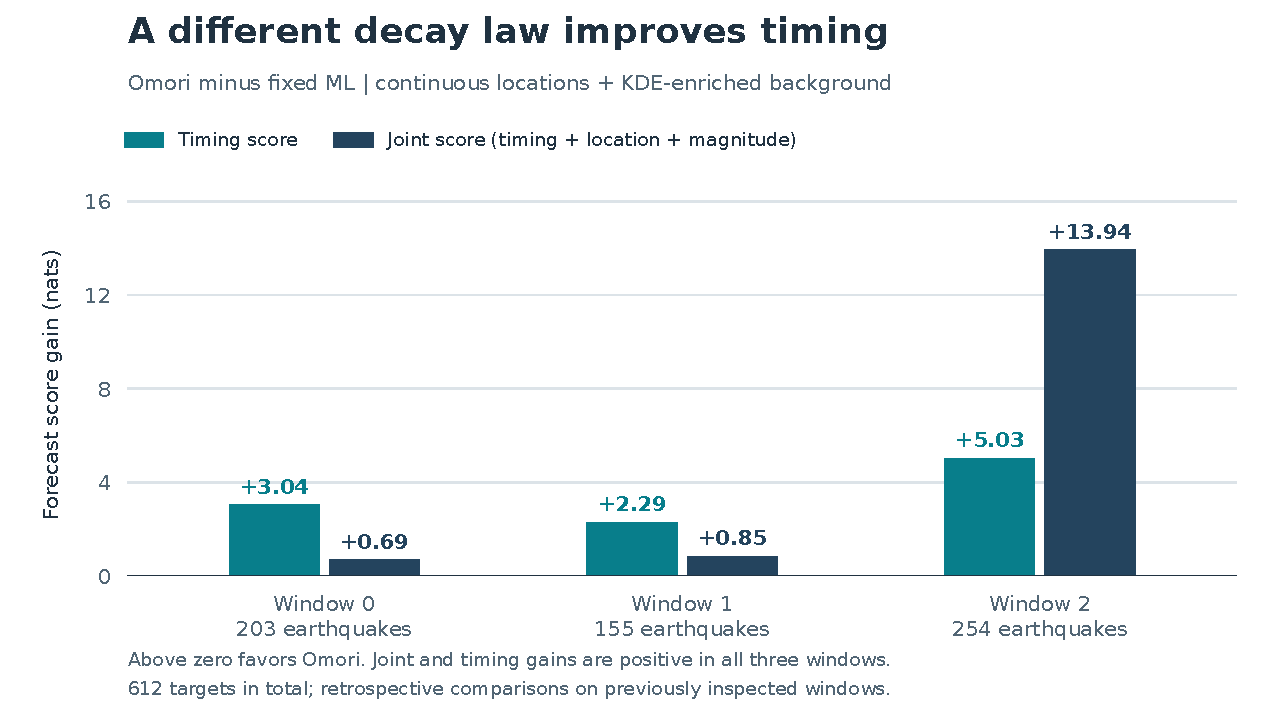
\includegraphics[width=\linewidth,height=.78\textheight,keepaspectratio]{spatial_addendum_iii_fig1_temporal.pdf}
\caption{Temporal comparisons across the three historical evaluation windows.}\end{figure}

\section{The location improvement survives stronger background geography}

Every continuous-minus-lift joint contrast wins all three windows under both backgrounds. The table below separates the spatial refinement from the effect of improving background geography. These contrasts are descriptive; no confidence intervals are supplied.

\begingroup\footnotesize\setlength{\tabcolsep}{2pt}\renewcommand{\arraystretch}{1.18}
\begin{longtable}{@{}>{\raggedright\arraybackslash}p{0.1800\textwidth}>{\raggedright\arraybackslash}p{0.1800\textwidth}>{\raggedright\arraybackslash}p{0.1800\textwidth}>{\raggedright\arraybackslash}p{0.1800\textwidth}>{\raggedright\arraybackslash}p{0.1800\textwidth}@{}}
\toprule
{}Temporal family & Continuous - lift, cell background (nats) & Continuous - lift, KDE-enriched background (nats) & KDE continuous--lift joint (nats/event) & KDE continuous--lift timing (nats) \\
\midrule\endfirsthead
\toprule
Temporal family & Continuous - lift, cell background (nats) & Continuous - lift, KDE-enriched background (nats) & KDE continuous--lift joint (nats/event) & KDE continuous--lift timing (nats) \\
\midrule\endhead
\midrule\multicolumn{5}{r}{\emph{Continued on next page}}\\
\endfoot
\bottomrule\endlastfoot
{}Fixed ML & +1453.29 & +1424.12 & +2.327 & +16.5456 \\
{}Common ML & +1445.7 & +1423.3 & +2.32565 & +15.1151 \\
{}Omori & +1507.21 & +1449.79 & +2.36893 & +27.8846 \\
\end{longtable}\endgroup

The stronger background reduces the continuous-location advantage by 22.397419-57.420970 nats. It explains some of that advantage, but does not remove it within the declared models.

Location dominates the remaining improvement. For Omori with KDE-enriched background, the +1449.785291 joint nats comprise +27.884617 timing, +14.810114 conditional-zone, +18.815997 conditional-cell and +1388.274563 within-cell area-density nats. Magnitude differences are zero. The timing aggregate is positive despite two losing windows (+35.932611, -2.308009, -5.739984); this spatial result must not be presented as uniform timing success.

Changing background geography itself improves continuous-model joint scores by 85.740055, 92.606919 and 33.248405 nats for fixed ML, common ML and Omori. For Omori that background change loses 1.757274 timing nats. At fixed common parameters, normalized spatial changes leave total regional intensity unchanged; their fitted timing effects arise through refitting.

\begin{figure}[htbp]\centering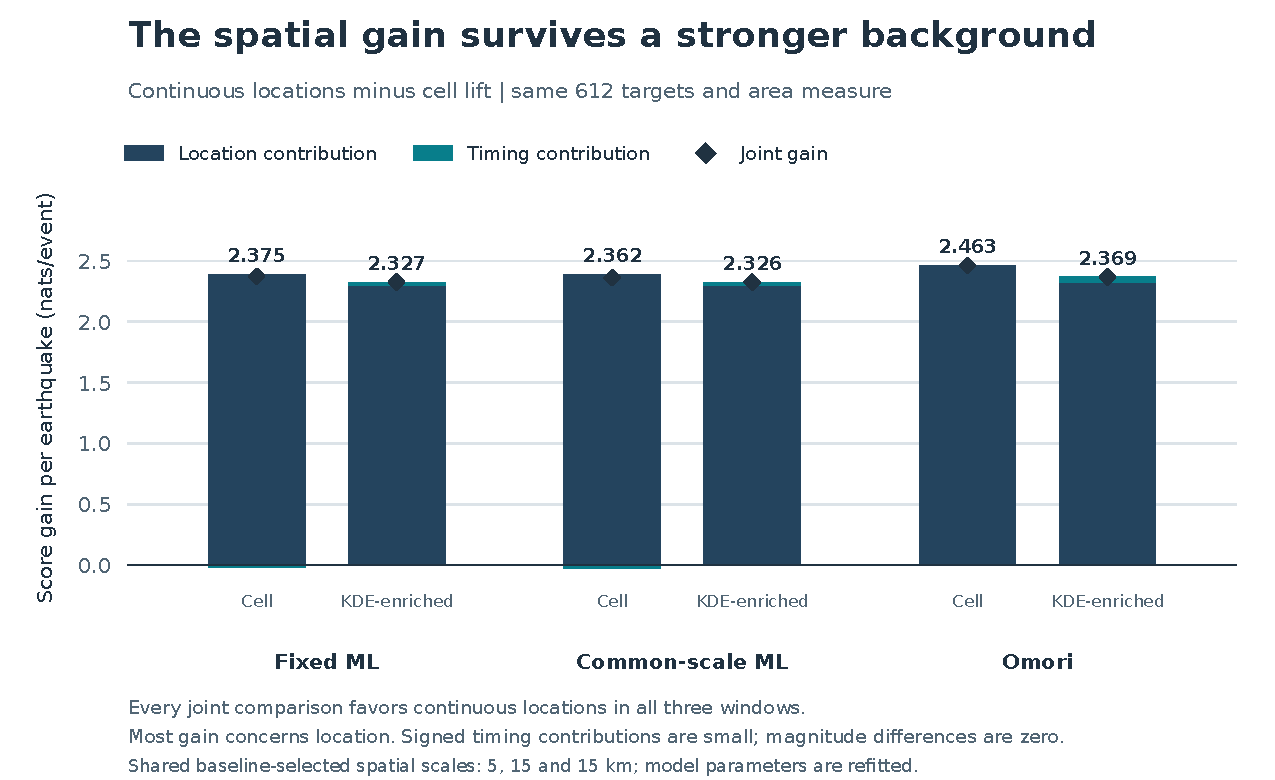
\includegraphics[width=\linewidth,height=.78\textheight,keepaspectratio]{spatial_addendum_iii_fig2_spatial.pdf}
\caption{Continuous-location improvements under both background representations, with location and timing distinguished.}\end{figure}

\section{Combined procedure and scale sensitivity}

Against the current matched fixed-ML/cell-background/lift comparator, Omori with continuous locations gains 1521.255407 joint nats using cell background, or 1554.503812 nats (2.540039 per event) using KDE-enriched background. The latter has +11.530195 timing nats and +1542.973617 net conditional-location nats; magnitude contributes zero. Joint gains are positive in all three windows, but timing changes are -2.961931, +4.108633 and +10.383493. These are direct fitted contrasts, not sums of earlier separate experiments. The previous sealed lift procedure selected its own sigma and is not the present shared-sigma comparator.

Training selected sigma values of 5, 15 and 15 km; KDE bandwidth was 15 km in all three windows. The first sigma lies at the primary grid's lower endpoint. Bounded sensitivity therefore retained separate fixed-ML/continuous fits at 1 and 2 km under both backgrounds. All twelve lost joint score against their primary reference, by 96.988003-308.063524 nats. Some improved timing while losing more location density. These sensitivity fits neither replace the primary models nor constitute an expanded-grid factorial.

\begin{figure}[htbp]\centering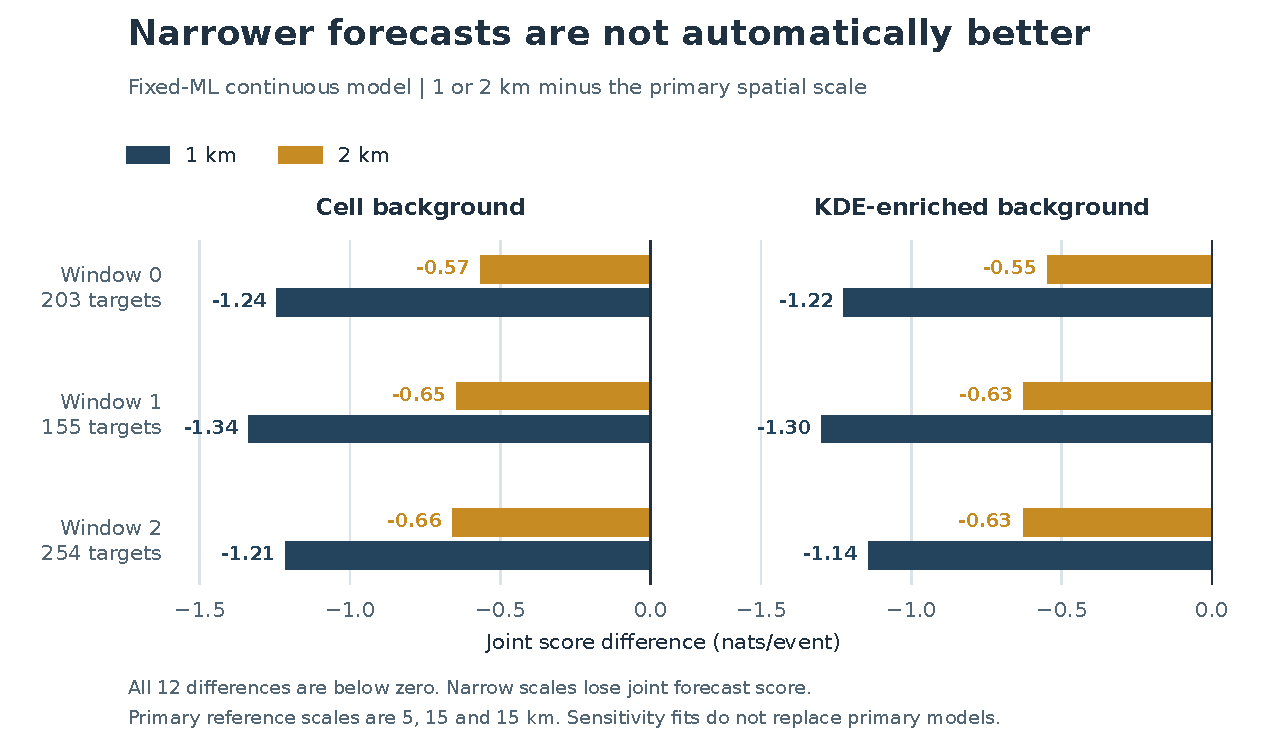
\includegraphics[width=\linewidth,height=.78\textheight,keepaspectratio]{spatial_addendum_iii_fig3_sensitivity.pdf}
\caption{Joint-score losses from the declared 1 and 2 km sensitivity procedures.}\end{figure}

The catalogue has 910 distinct coordinate pairs among 913 events, with three repeated pairs. Serialized decimal places do not establish location accuracy; these results identify neither a physical interaction distance nor a universal optimal bandwidth.

\section{Validation, scope and implications}

All 63 observed procedures and 504 prescribed starts resolved, retaining 579 candidates and 75 exact floors. Including two fixed-seed engineering histories, totals are 87 procedures, 696 starts and solver returns, 803 candidates and 107 floors. Analytic gradients, finite differences, normalization, exact nesting and quadrature checks preceded observed fitting. An independent raw-history auditor reconciled saved scores to within 3.28e-11 nats, below the unchanged 1e-4 tolerance. Near-optimal forecast spread passed the declared gate. Neither multiple starts nor that gate certifies a global optimum.

One initial audit failed because a metadata assertion required exact binary equality between independently solved magnitude-rate estimates differing by six floating-point units. An append-only repair separated exact producer identity from the existing reconstruction tolerance. Independent numerical scores still used raw-derived values; all 326 scientific outputs remained unchanged, with no refits or replacement histories. The audit review and accounting retain that failure and recovery. The reconstructed catalogue rows are now supplied with an executable cohort replay; event-level feature caches are numerical rebuild products. This chapter retains its reviewed spatial aggregates and does not claim a new execution of these spatial fits or their original score audit. Computational-agent review is not external academic peer review.

The strongest supported conclusion is a positive retrospective forecasting ablation: finer offspring-location representation retains a large location-score advantage under a stronger background, while Omori adds a smaller timing improvement against fixed ML in the continuous model. Background and temporal comparisons also contain losses that prevent a blanket preference claim. Constant-Poisson floors are numerical witnesses, not an optimized no-trigger comparator, so this experiment does not establish that physical triggering is present or required. It does not test inhibition.

The same historical windows have been inspected repeatedly; overlapping training prefixes and dependent earthquake histories preclude event-iid confidence intervals or claims of independent replication. Proper held-out scoring does not remove this adaptive-reuse limitation. No Wilks inference, physical causality, immigrant-law recovery or universal scale claim follows. At the time of this factorial study, continuous local inhibition and unused-data replication were design-only follow-ons. The subsequently completed immigrant-only local-inhibition study is reported in Chapter~\ref{ch:local-inhibition}; genuinely unused-data replication remains a separate objective. The current update supplies a bounded positive predictive finding while preserving those outstanding questions and all earlier manuscript conclusions in their original scope.
% Audit-table relocation: app:audit10-factorial
All primary arm-by-window absolute scores are retained in Appendix~\ref{app:audit10-factorial}; its \hyperref[app:audit10-sensitivity]{small-scale sensitivity table} retains every bounded sensitivity fit.

\section{Reproducible geometry and fitting contract}
Let $A_c$ be projected cell area and $N_c,N_z$ the training cell and zone counts. The hierarchical reference obeys
\begin{equation}
 \pi_z=N_z/N,\qquad q(c\mid z)=\frac{N_c+1/2}{N_z+3/2},\qquad
 b_{\rm ref}(z)=\frac{\pi_{z(c)}q(c\mid z(c))}{A_c}\quad(z\in c).
\end{equation}
Writing $D_h(v)=(1+\lVert v\rVert^2/h^2)^{-2}$, define $F_j(h)=\int_D D_h(v-z_j)\,\mathrm dv$. The actual smooth immigrant density and the parent-normalized offspring law are
\begin{align}
 b_{\rm bg}(z)&=0.05b_{\rm ref}(z)+\frac{0.95}{N}\sum_{j=1}^N\frac{D_h(z-z_j)}{F_j(h)},\\
 s_\sigma(z\mid z_j)&=\frac{b_{\rm ref}(z)D_\sigma(z-z_j)}{\int_D b_{\rm ref}(v)D_\sigma(v-z_j)\,\mathrm dv},\\
 W_{cj}&=\frac{\pi_cD_\sigma(v_c-z_j)}{\sum_l\pi_lD_\sigma(v_l-z_j)},\qquad
 s_{\rm lift}(z\mid z_j)=W_{cj}/A_c\quad(z\in c).
\end{align}
Here $v_c$ is the projected rectangle centre and $\pi_c=\pi_{z(c)}q(c\mid z(c))$. Parents retain actual coordinates in both laws; only the lift's target weights use centres. The same KDE-enriched immigrant density is retained even in a lifted offspring arm; its cell-density floor can retain boundary jumps. Leave-one-out selection removes the scored row's identity from both the kernel mixture and hierarchical counts, retains other observations with duplicate coordinates, and normalizes every retained kernel separately. Exact bandwidth ties select the smaller bandwidth. Full-training plug-in nuisance density, including self contributions, is frozen after selection.

The equal-area coordinates are $x=R\cos\phi_0(\lambda-\lambda_0)$ and $y=R(\sin\phi-\sin\phi_0)/\cos\phi_0$, with angular arguments in radians. Euclidean radial isotropy is specific to this projection. Multiplication by piecewise reference geography and finite-domain truncation generally destroys isotropy and translation invariance of the full density. Positive rectangle integrals are checked without clipping invalid values. For any parent, finite-window temporal exposure uses $S(L)-S(U)$ with $L=\max(t_{\rm start}-t_j,0)$ and $U=\max(t_{\rm end}-t_j,0)$; temporal kernels are never renormalized to the evaluation window.

All main fits use the same bounded training-likelihood selection rule. Fixed ML starts span the prescribed amplitude offset, trend and branching schedule. Common-scale ML and Omori initialize shared nuisance coordinates from their same-background/same-geography fixed-ML fit; this is a declared procedure dependency, not held-out selection. The constant-Poisson floor is an admissible numerical witness. Common-scale ML additionally retains the exact fixed-ML floor; Omori and ML are not nested within these finite parameter bounds. Background and continuous/lift families are not declared nested.
% Audit-table relocation: app:audit10-protocol
The complete scalar numerical protocol, prescribed starts, bounds and engineering-control coordinates are retained in Appendix~\ref{app:audit10-protocol}.

